\documentclass[12pt,a4paper,twoside]{mwart}
\usepackage[T1]{fontenc}
\usepackage[utf8]{inputenc}
\usepackage{polski} \usepackage{indentfirst}
\usepackage[left=3cm,right=2cm,top=2.5cm,bottom=2.5cm]{geometry}
\usepackage{todonotes}
\usepackage{listings}
\usepackage{float}
\usepackage{hyperref}
\usepackage{dirtree}
\usepackage{fancyhdr}
\usepackage[nottoc,numbib]{tocbibind}
\usepackage{apacite}
\usepackage{enumitem}

\setlength{\parskip}{13pt plus 2pt minus 3pt} %% Odstęp dla paragrafów
%% \linespread{1.15} odstep pomiędzy liniami?

\newcommand{\makecell}[2][@{}c@{}]{\begin{tabular}{#1}#2\end{tabular}}
\newcommand{\file}[1]{\textbf{\textit{\textcolor{darkgreen}{#1}}}}
\newcommand{\folder}[1]{\textbf{\textit{\textcolor{dodgerblue}{#1}}}}

\pagestyle{fancy}
%% JN: nie jestem pewien czy klasa 'article' z 'openany' ma \markright
%% JN: uproszczenie paginy: tylko autor i tytuł pracy, zamiast tytułu
%%     bieżącego rozdziału.
\renewcommand{\sectionmark}[1]{\markright{#1}}
\fancyhf{}
\fancyhead[LO]{\small \emph{\nouppercase{\leftmark}}}
\fancyhead[RE]{\small \emph{\nouppercase{\rightmark}}}

\cfoot{\fancyplain{}{\thepage}}

% Czesc odpowiedzialna za styl kodu
% Taken from Lena Herrmann at 
% http://lenaherrmann.net/2010/05/20/javascript-syntax-highlighting-in-the-latex-listings-package
\usepackage{listings}
\usepackage{color}
\definecolor{lightgray}{rgb}{.9,.9,.9}
\definecolor{darkgray}{rgb}{.4,.4,.4}
\definecolor{purple}{rgb}{0.65, 0.12, 0.82}
\definecolor{dodgerblue}{RGB}{28, 134, 238}
\definecolor{darkgreen}{RGB}{0,153,51}
\definecolor{darkOrange}{RGB}{120,30,0}

\lstdefinelanguage{JavaScript}{
  keywords={typeof, new, true, false, catch, function, return, null, try, catch, switch, var, let, if, in, while, do, else, case, break},
  keywordstyle=\color{purple}\bfseries,
  ndkeywords={class, export, boolean, throw, implements, import, this, Math, Float32Array, Array},
  ndkeywordstyle=\color{blue}\bfseries,
  identifierstyle=\color{black},
  sensitive=false,
  comment=[l]{//},
  morecomment=[s]{/*}{*/},
  commentstyle=\color{darkgreen}\ttfamily,
  stringstyle=\color{darkOrange}\ttfamily,
  morestring=[b]',
  morestring=[b]"
}

\lstset{
   language=JavaScript,
   backgroundcolor=\color{lightgray},
   extendedchars=true,
   basicstyle=\footnotesize\ttfamily,
   showstringspaces=false,
   showspaces=false,
   %% JN: jeśli ie odwołuje się do konkretnych linii, to ich numerowanie nie do końca ma sens
   %% JN: jesli numerowanie linii jest uzywane do pokazania gdzie linie zostały zawiniete,
   %%     to lepiej uzyć mniej agresywnego stylu
   numbers=left,
   numberstyle=\footnotesize,
   numbersep=9pt,
   tabsize=2,
   breaklines=true,
   showtabs=false,
   captionpos=b
}

\setlength {\marginparwidth }{2cm}
\begin{document}
  
\begin{titlepage}
	\begin{center}
		\large Uniwersytet Mikołaja Kopernika w Toruniu\\
		\large Wydział Matematyki i Informatyki\\
		\vspace{3cm} 
		\large Patryk Bieszke\\
			nr albumu: 273187\\
			informatyka\\
		\vspace{2cm}
		Praca magisterska\\
	
		\vspace{3cm} 
		\huge Generowanie kompozycji muzycznych z użyciem sieci neuronowych\\
	\end{center}
	\hfill
	\begin{minipage}{6cm}
		\vspace{3cm}
		Opiekun pracy dyplomowej\\
		prof. dr hab. Krzysztof Stencel
	\end{minipage}
	\vspace{4cm}
	\begin{center}
		Toruń 2018\\
	\end{center}
\end{titlepage}


\pagenumbering{gobble}% Remove page numbers (and reset to 1)

\bibliographystyle{apacite}
\bibliography{References}
\clearpage
\thispagestyle{empty}
\mbox{}

\pagenumbering{arabic}
\tableofcontents 

\clearpage

\setcounter{secnumdepth}{0}
\section{Wstęp}
\label{sec:wstep}

\newpage

\section{Słownik skrótów}
\begin{itemize}
\item \textbf{DAW} - \textit{ang. \textbf{D}igital \textbf{A}udio \textbf{W}orkstation}, pol. Cyfrowa Stacja Robocza 
\item \textbf{MIDI} - \textit{ang. \textbf{M}usical \textbf{I}nstrument \textbf{D}igital \textbf{I}nterface}
\item \textbf{AUX} - \textit{ang. \textbf{Aux}iliary}
\item \textbf{W3C} - \textit{ang. \textbf{W}orld \textbf{W}ide \textbf{W}eb \textbf{C}onsortium}
\item \textbf{SVG} - \textit{ang. \textbf{S}calable \textbf{V}ector \textbf{G}raphics}
\item \textbf{HTML} - \textit{ang. \textbf{H}yper\textbf{t}ext \textbf{M}arkup \textbf{L}anguage}
\item \textbf{CSS} - \textit{ang.  \textbf{C}ascading \textbf{S}tyle \textbf{S}heets}
\item \textbf{JS} - \textit{\textbf{J}ava\textbf{S}cript}
\item \textbf{DOM} - \textit{ang. \textbf{D}ocument \textbf{O}bject \textbf{M}odel}
\item \textbf{API} - \textit{ang. \textbf{A}pplication \textbf{P}rogramming \textbf{I}nterface}
\item \textbf{CLI} - \textit{ang. \textbf{C}ommand \textbf{L}ine \textbf{I}nterface}
\item \textbf{CQRS} - \textit{ang. \textbf{C}ommand \textbf{Q}uery \textbf{R}esponsibility \textbf{S}egregation}
\item \textbf{MVC} - \textit{ang. \textbf{M}odel-\textbf{V}iew-\textbf{C}ontroller}
\item \textbf{URL} - \textit{(ang. \textbf{U}niform \textbf{R}esource \textbf{L}ocator )}
\item \textbf{npm} - \textit{(ang. \textbf{N}ode \textbf{P}ackage \textbf{M}anager)}
  \todo[inline]{Czy jest to dobra konwencja dla słownika skrótów? Czy umieścić go przed wstępem z racji tego, że we wstępie chciałbym użyć DAW?}
  
\end{itemize}
\newpage
\setcounter{secnumdepth}{2}

\section{Transkrypcja muzyki}
Pliki dźwiękowe przechowują sygnały foniczne w postaci sygnałów cyfrowych. Układ, w którym pliki te przechowują bity jest zdeterminowany przez kodowanie, które zostało na nich zastosowane. Istnieje wiele kodowań przeznaczonych do danych dźwiękowych, zarówno nieskompresowanych jak i skompresowanych. Te drugie powtały z myślą o zaoszczędzeniu jak największej ilości pamięci w zaleności od tego, w jakim stopniu mona pójść na kompromis z jakością skompresowanego sygnału.

Z punktu widzenina algorytmów generujących muzkę, w tym modeli sieci, pliki dźwiękowe nie są wystarczająco funkcjonalną formą trzymania danych. W celu pozyskania istotnych informacji w kontekście maszynowej kompozycji muzyki należałoby zastosować szereg algorytmów, w tym transformacji i funkcji statystycznych, na każdym z plików. Proces ten jest skomplikowany pod względem obliczeniowym, co w połączeniu z dużym woluminem danych czyni go czasochłonnym. Z racji tego, że kategoryzacje zbioru muzycznego jak i dynamiczne dostosowywanie modelu, na podstawie którego zostaną generowane kompozycje muzyczne według założeń projektu ma odbywać się w czasie rzeczywistym, jedyną formą przechowywania plików z informacją o kompozycjach będzie postać po zastosowaniu transkrypcji na danych utworach.

%% z PWN : transkrypcja [łac. transcriptio ‘przepisywanie’], muz. opracowanie utworu muz. na inny niż w oryginale zespół wykonawczy (orkiestracja) lub inny instrument; Pytanie czy rozszerzenie tego znaczenia w języku polskim jest poprawne? także zapisanie utworu inną notacją muz.; transkrybować — zapisywać znakami współcz. notacji muz. utwory zapisane dawnymi systemami notacyjnymi, np. notacją modalną, menzuralną. Po ENG transkrypcja jest zgodna z rozdziałem

Transkrypcja muzyki to proces polegający na zapisaniu danego utworu muzycznego w sposób formalny, taki jak zapis nutowy, z istniejącego zapisu dźwiękowego. Operacja ta wykorzystywana jest do lepszego zrozumienia muzyki, która wcześniej nie była zapisana w taki sposób. Jest to skomplikowany i czasochłonny proces nawet dla profesjonalistów z dużym doświadczeniem w tej dziedzinie. Algorytmiczne podejście do tego problemu obejmuje rozpoznanie rytmu i wysokości tonu poprzez analize sygnału fonicznego. Do polepszenia rezultatu tego procesu często wymagane jest odesparowanie od siebie poszczególnych instrumentów w danym utworze muzycznym, ponieważ nakładanie się na siebie sygnały odrębnych źródeł stanowi jeden z większych problemów transkrypcji

W tym rozdziale przedstawię wciąż nierozwiązany problem automatycznej transkrypcji muzycznej, nakreślając najbardziej problematyczne rejony na przykładach istniejących rozwiazań.  Celem tych rozważań jest przybliżenie działania modułu opisywanego projektu, służącego do transpilacji wysłanego przez użytkownika pliku dźwiękowego

\subsection{Jak "działa" muzyka}
Uproszczając pojęcie muzyki, są to dźwięki podniesione do odpowiednich wysokości z zachowaniem odpowiedniego rytmu. Wysokości tych dźwięków są proporcjonalne do częstotliwości wibracji, które zostały wytworzone przez dany instrument czy głos ludzki. Starając się rozłożyć skomplikowaną strukturę utworów muzycznych na częsci pierwsze, można wyróżnić cztery esencjalne składowe, których zbadanie i zinterpretowanie jest przedmiotem algorytmów muzycznych. Są to:
\begin{itemize}
\item Rytm
\item Wysokość tonu
\item Głośność
\item Barwa dźwięku
\end{itemize}
Składowe te są widoczne bardzo wyraźnie w zapisie nutowym, z kolei ten jest wystarczającym źródłem informacji dla muzyków aby zagrać dany utwór muzyczny. Zapisane nuty przedstawiają wysokość tonu jak i jego barwę wraz z długością granego dźwięku i poziomem głośności jaki powinien zostać zastosowany. Innymi, wysoko praktycznymi informacjami, do których dostęp daje muzykom zapis nutowy, są: 
\begin{itemize}
  \item tempo utworu, czyli szybkość z jaką nuty powinny być grane, 
  \item sygnatura czasowa, która wyznacza bazową strukture rytmiczną w jakiej dany utwór został napisany,
  \item klucz w którym został napisany utwór, opisujący harmoniczną podstawę kompozycji, co w praktyce ogranicza dostępne wysokości tonu.
\end{itemize} 
Informacją, którą zapis nutowy nie zapewnia, jest barwa dźwięku. Parametr ten jest ściśle związany z instrumentem, którego dotyczy dany dźwięk, ponieważ każde ze źródeł dźwięku cechuje się odrębną barwą, nawet gdy uwzględnić taką samą wysokość i głośność sygnału fonicznego. Problem rozróżniania tej cechy jest zwiazany z transkrypcją muzyki, jak i algorytmami identyfikującymi instrumenty poprzez analizę barwy dźwięku.

W dalszej kolejności zostaną pokrótce opisane cztery wymienione wyżej cechy, które są głównym przedmiotem analizy w kierunku transkrypcji muzycznej.

\subsubsection{Rytm}
W kontekście muzykologji, rytm jest bazową struktórą czasową utworu. Nie można niestety zakładać stałości rytmu na przestrzeni całego utworu, ponieważ powszechną praktyką jest jego modyfikacja w trakcie trwania wykonania w celu uzyskania specyficznych efektów artystycznych. Bardzo częstą praktyką jest na przykład minimalne podnoszenie tempa na czas każdego z refrenów w celu ich wypuklenia na tle całości kompozycji.

Podstawową jednostką rytmiczną jest nuta. Miarą tempa utworu przeniesioną na domenę fizyczną są \textbf{uderzenia na minutę} \textit{(ang. beats per minute, BPM)} oznaczające liczbę ćwierćnut przypadających na jedną minutę. \textbf{Taktem} nazywamy odcinek zapisu muzycznego wizualnie oznaczony pionowymi kreskami. Takty tworzą regularne odcinki czasowe, a ich długość jest zależna od \textbf{metrum}. Metrum jest oznaczeniem metrycznym opisującym ile jakich jednostek mieści się w takcie. Dla przykłądu, najpopularniejszym metrum w muzyce pop jest 4/4, co oznacza, że w każdym takcie mieszczą się cztery ćwierć nuty.
\begin{figure}[H]
\begin{center}
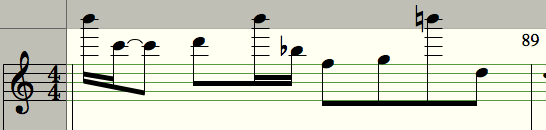
\includegraphics[scale=0.5]{images/Rytm_pieciolinia.png}\\
(Przykład użycia React Developer Tools w przeglądarce Chrome)
\end{center}
\end{figure}

\subsubsection{Głośność}
Jak głośno 

\subsection{Transformata Fouriera}

\subsection{Estymacja składowej fundamentalnej}

\subsection{Estymacja wielotonowa}


\newpage
\section{Klasyfikacja muzyki}

\section{Generowanie muzyki}

\section{Implementacja}

\section{Zakonczenie}

OKok
\end{document}  
